

\section{Forward Kinematics}
Forward kinematics is used for calculating the position and orientation of the end-effector of a robotic manipulator. This can be done by using the matrices describing the position and orientation of each of the joints of the specific robotic manipulator, and the following formula: \\

\begin{equation}
    _N^0 T = _1^0T  _2^1T  _3^2T  _4^3T  .........  _N^N^-^1T\\
\end{equation} \\

This is the formula used for calculating the end-effector of a robotic manipulator. \\

Now, the required transformation matrices can simply be inserted into the formula, and the matrix describing the position of the end-effector can be calculated. \\

So the main idea is, given the joint angles as input, you would be able to get the coordinates for the end-effector as output. So the position can be calculated from specific set values, and used for simulations.  \\

Kinematics can be used to form an internal picture of the robot movements, and help understanding and explaining it. 

This is useful when working with not only manipulators, but also animations in movies and video games, or any other movement where multiple joints are used. 

\section{Denavit-Hartenberg}

In order to enable the UR5 on the flexible workstation to locate itself and its surroundings within a space, the DH (Denavit-Hartenberg) method is used.\\ 
The DH method can be used to compute every frame into parameters.\\
These descriptions of the system can be used to translate every point and every movement of the robotic manipulator, with the help of forward kinematic.\\
Initially the start is to locate all of the coordinate systems, as seen in \ref{table:DH-table}.\\ 


\begin{itemize}
    \item ${a_{i-1}}$= The distance from ${Z_{i-1}}$ to ${Z_{i}}$ measured along ${X_{i-1}}$
    \item ${\alpha_{i-1}}$ = The angel between ${Z_{i-1}}$ to ${Z_{i}}$ measured about ${X_{i-1}}$
    \item ${d_{i}}$ = The distance from ${X_{i-1}}$ to ${X_{i}}$ measured along ${Z_{i}}$
    \item ${\theta_{i-1}}$ = The angel between ${X_{i-1}}$ to ${X_{i}}$ measured about ${Z_{i}}$
\end{itemize}




Then the angles and the distance from each coordinate system is computed and set in to a table as seen in \ref{fig:DH-Table}.

\begin{figure}[h!]
    \centering
    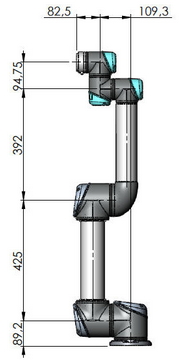
\includegraphics[scale=0.79]{Design/UR5measure.png}
    \caption{UR5 to describing DH-parameters \cite{DH}} 
    \label{fig:DH-Table} 
\end{figure}

%\begin{table}[h!]
%\centering
%\begin{tabular}{||c c c c c||} 
% \hline
% i & \alpha_{i-1} & a_{i-1} & d_{i} & \theta_{i} \\ [0.5ex] 
% \hline\hline
% 1 & 0 & 0  & 0     & \theta_{1} \\ 
% 2 & 0 & l_{1} & 0 & \theta_{2} \\
% 3 & 0 & l_{2} & 0 & \theta_{3} \\[1ex]
% \hline
%\end{tabular}
%\caption{DH-Table}
%\label{table:DH-table}
%\end{table}

As seen in \ref{fig:DH-Table},the coordinate systems is used to trace every step of each axis.\\
Starting from left to right at the top of the table, the $\alpha-1$ is used to compute the differences of the angles between $Z_{i}$ and $Z_{i-1}$, which is 0, due to the fact that they keep the same angle from $Z_{i}$  to $Z_{i-1}$.\\
It can also be seen from the table that the distance between $Z_{i}$ and $Z_{i-1}$ is Length2, since they are parallel to each other.\\ 
The distance between $X_{i-1}$ and $X_i$ is 0 since they cross each other on the perpendicular line, which means that in that point the new coordinate system should be placed.\\

\begin{table}[h!]
\centering
\begin{tabular}{||c c c c c||} 
 \hline
 i & \alpha_{i-1} & a_{i-1} & d_{i} & \theta_{i} \\ [0.5ex] 
 \hline 
 \hline
 1 & 0 & 0 & 89.2 & \theta_{1} \\ 
 2 & 90 & 0 & 0 & \theta_{2} \\
 3 & 0 & 425 & 0 & \theta_{3} \\
 4 & 0 & 392 & 109.3 & \theta_{4} \\
 5 & 90 & 0 & 94.75 & \theta_{5} \\ 
 6 & -90 & 0 & 82.5 & \theta_{6} \\[1ex] 
 \hline
\end{tabular}
\caption{DH-parameters for the UR5, using \cite{DHPar} as measurement.}
\label{table:1}
\end{table}

\section{Inverse Kinematics}
Inverse kinematics is used to compute the joint angles from a given position and orientation of an object\cite{JohnC}. The inverse kinematic can be set up from two aspects, one is the geometric way and the other is an algebraic solution, the one the team is using is the algebraic solution where the inverse kinematics is set up in MATLAB, a math computer program, where it makes it possible to be used later in computing the trajectory of the manipulator.\\
\section{Conclusion}

Describing a robot with forward kinematics and Denavit-Hartenberg parameters is used to locate the different joints and the tool in 3D-space, so the robot can be manipulated and used for various tasks.\\
Looking at Denavit-Hartenberg, the advantage of this method is to simplify the different axis in a matrix, so the operator and the robot can identify where the different coordinate systems is located.\\
Forward kinematics is the starting point of selecting the DH-parameters, when we know the point $Z_{1-1}$ and $Z_1$ we can then locate every axis in the desired robot. Hereby conclude to DH-parameters and include them into MATLAB while visualizing the robot and locate the robot so the tasks can be performed.\\